\section{Software: Composyx}
\label{sec:Composyx:software}

\begin{table}[h!]
    \centering
    { \setlength{\parindent}{0pt}
    \def\arraystretch{1.25}
    \arrayrulecolor{numpexgray}
    {\fontsize{9}{11}\selectfont
    \begin{tabular}{!{\color{numpexgray}\vrule}p{.4\textwidth}!{\color{numpexgray}\vrule}p{.6\textwidth}!{\color{numpexgray}\vrule}}
        \rowcolor{numpexgray}{\rule{0pt}{2.5ex}\color{white}\bf Field} & {\rule{0pt}{2.5ex}\color{white}\bf Details} \\
        \rowcolor{white}\textbf{Consortium} & \begin{tabular}{l}
None\\
\end{tabular} \\
        \rowcolor{numpexlightergray}\textbf{Exa-MA Partners} & \begin{tabular}{l}
Inria BXSO\\
\end{tabular} \\
        \rowcolor{white}\textbf{Contact Emails} & \begin{tabular}{l}
gilles.marait@inria.fr\\
\end{tabular} \\
        \rowcolor{numpexlightergray}\textbf{Supported Architectures} & \begin{tabular}{l}
CPU Only\\
\end{tabular} \\
        \rowcolor{white}\textbf{Repository} & \href{https://gitlab.inria.fr/composyx/composyx}{https://gitlab.inria.fr/composyx/composyx} \\
        \rowcolor{numpexlightergray}\textbf{License} & \begin{tabular}{l}
OSS: Cecill-*\\
\end{tabular} \\
        \rowcolor{white}\textbf{Bottlenecks roadmap} & \begin{tabular}{l}
B10 - Scientific Productivity\\
B11 - Reproducibility and Replicability of Computation\\
B6 - Data Management\\
B7 - Exascale Algorithms\\
\end{tabular} \\
        \bottomrule
    \end{tabular}
    }}
    \caption{Composyx Information}
\end{table}

\subsection{Software summary}
\label{sec:Composyx:summary}
Composyx (previously  Maphys++) is a linear algebra C++20 library focused on composability. Its purpose is to allow the user to express a large panel of algorithms using a high-level interface to range from laptop prototypes to many node supercomputer parallel computations.
Currently it mostly implements domain decomposition methods as described in~\cite{agullo_robust_2019} using hybrid parallel implementation (MPI+Thread, MPI+StarPU) to address heterogeneous manycores.

\begin{figure}
        \centering
        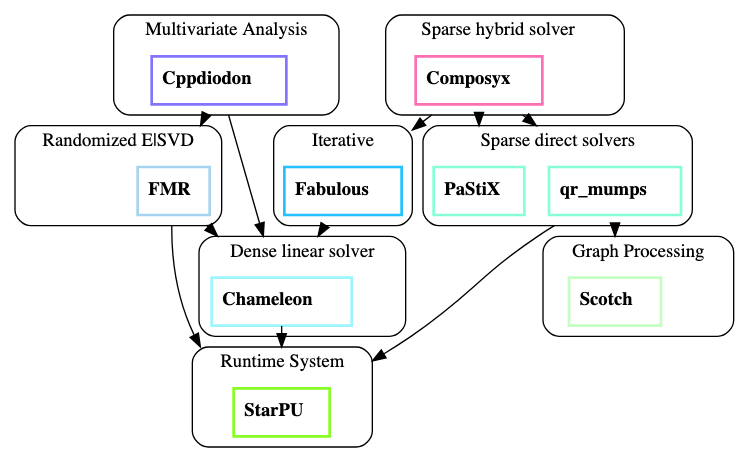
\includegraphics[width=0.8\textwidth]{graphics/composyx/composyx-solverstack.png}
        %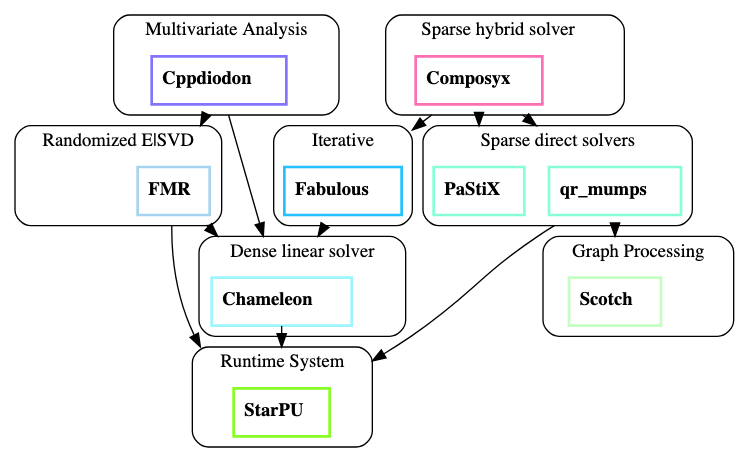
\includegraphics[width=0.8\textwidth]{graphics/composyx/composyx-solverstack.pdf}
        \caption{Composyx dependencies}
        \label{fig:composyx}
    \end{figure}

\subsection{Purpose}
\label{sec:Composyx:purpose}
Solution of large sparse linear systems using preconditioned subspace methods. For that purpose it relies on the Fabulous packages that implements various techniques including block variants for multiple right-hand sides~\cite{giraud_block_2022}

\subsection{Programming and Computational Environment}
\label{sec::Composyx:environment_capabilities}


The following table summarizes these aspects for Composyx, providing a  view of its programming and computational capabilities.

\begin{table}[h!]
    \centering
    {
    \setlength{\parindent}{0pt}
    \def\arraystretch{1.25}
    \arrayrulecolor{numpexgray}
    {\fontsize{9}{11}\selectfont
    \begin{tabular}{lp{.3\textwidth}p{.5\textwidth}}
        \rowcolor{numpexgray}{\rule{0pt}{2.5ex}\color{white}\bf Category}  & {\rule{0pt}{2.5ex}\color{white}\bf Details} & {\rule{0pt}{2.5ex}\color{white}\bf Description}\\
        \rowcolor{white}Languages  & \begin{tabular}{l}
C\\
C++20\\
Fortran\\
\end{tabular} & Programming languages and language standards supported by the software \\
        \rowcolor{numpexlightergray}Parallelism  & \begin{tabular}{l}
GPU\\
MPI\\
Multithread\\
\end{tabular} & Multithreading OpenMP and Posix, hybrid CPU-GPU with StarPU.\\
%\rowcolor{white}Data Formats  & \begin{tabular}{l} None\\ \end{tabular} & Data formats that the software can handle or produce.\\
%\rowcolor{numpexlightergray}Resilience  & \begin{tabular}{l} None\\ \end{tabular} & \\
\rowcolor{white}DevOps & \begin{tabular}{l} Continuous Integration\\ \end{tabular} & Outlines the development and operational practices including continuous integration, containerization, and testing methodologies.  \\
%
\rowcolor{numpexlightergray}Packaging  & \begin{tabular}{l} GUIX-HPC\\ \end{tabular} & Software packaging and distribution.\\ 
\rowcolor{white}Testing  & \begin{tabular}{l} Verification\\ \end{tabular} & Testing methodologies employed to ensure software quality and correctness.\\
\rowcolor{numpexlightergray}Containerization  & \begin{tabular}{l} Singularity\\ \end{tabular} & Container technologies used to package and deploy the software.\\
\rowcolor{white}Interfaces  & \begin{tabular}{l} MUMPS\\ PaStiX\\ Scotch\\ qr\_mumps\\ \end{tabular} & List of software Composyx has interfaces with.\\
        \bottomrule
    \end{tabular}
    }}
    \caption{Composyx programming and computational environment}
\end{table}



%\subsection{Mathematics}
%\label{sec:Composyx:mathematics}
%Mathematics not available.

%In this section, provide a summary the mathematics used in the software.


\subsection{Relevant Publications}
\label{sec:Composyx:publications}

Here is a list of relevant publications related to the software:
\begin{description}
        \item[\fullcite{agullo_robust_2019}]
        The solution of large sparse linear systems is one of the most time consuming kernels in many numerical simulations. The domain decomposition community has developed many efficient and robust methods in the last decades. While many of these solvers fall into the abstract Schwarz (aS) framework, their robustness was originally demonstrated on a case-by-case basis. In this paper, we propose a bound for the condition number of all deflated aS methods provided that the coarse grid consists of the assembly of local components that contain the kernel of some local operators. We show that classical results from the literature on particular instances of aS methods can be retrieved from this bound. We then show that such a coarse grid correction can be explicitly obtained algebraically via generalized eigenproblems, leading to a condition number independent of the number of domains. This result can be readily applied to retrieve or improve the bounds previously obtained via generalized eigenproblems in the particular cases of Neumann-Neumann (NN), additive Schwarz (AS), and optimized Robin, but it also generalizes them when applied with approximate local solvers. Interestingly, the proposed methodology turns out to be a comparison of the considered particular aS method with generalized versions of both NN and AS for tackling the lower and upper part of the spectrum, respectively. We furthermore show that the application of the considered grid corrections in an additive fashion is robust in the AS case although it is not robust for aS methods in general. In particular, the proposed framework allows for ensuring the robustness of the AS method applied on the Schur complement, either with deflation or additively, and with the freedom of relying on an approximate local Schur complement. Numerical experiments illustrate these statements.
    \item[\fullcite{agullo_soft_2020}]
    The conjugate gradient (CG) method is the most widely used iterative scheme for the solution of large sparse systems of linear equations when the matrix is symmetric positive definite. Although more than 60 years old, it is still a serious candidate for extreme-scale computations on large computing platforms. On the technological side, the continuous shrinking of transistor geometry and the increasing complexity of these devices affect dramatically their sensitivity to natural radiation and thus diminish their reliability. One of the most common effects produced by natural radiation is the single event upset which consists in a bit-flip in a memory cell producing unexpected results at the application level. Consequently, future extreme-scale computing facilities will be more prone to errors of any kind, including bit-flips, during their calculations. These numerical and technological observations are the main motivations for this work, where we first investigate through extensive numerical experiments the sensitivity of CG to bit-flips in its main computationally intensive kernels, namely the matrix-vector product and the preconditioner application. We further propose numerical criteria to detect the occurrence of such soft errors and assess their robustness through extensive numerical experiments.
    \item[\fullcite{giraud_block_2022}]
        We are concerned with the iterative solution of linear systems with multiple right-hand sides available one group after another with possibly slowly varying left-hand sides. For such sequences of linear systems, we first develop a new block minimum norm residual approach that combines two main ingredients. The first component exploits ideas from GCRO-DR~\cite{parks_recycling_2006}, enabling us to recycle information from one solve to the next. The second component is the numerical mechanism for managing the partial convergence of the right-hand sides, referred to as inexact breakdown detection in IB-BGMRES~\cite{robbe_exact_2006}, that enables the monitoring of the rank deficiency in the residual space basis expanded blockwise. Next, for the class of block minimum norm residual approaches that relies on a block Arnoldi-like equality between the search space and the residual space (e.g., any block GMRES or block GCRO variants), we introduce new search space expansion policies defined on novel criteria to detect the partial convergence. These novel detection criteria are tuned to the selected stopping criterion and targeted convergence threshold to best cope with the selected normwise backward error stopping criterion, enabling us to monitor the computational effort while ensuring the final accuracy of each individual solution. Numerical experiments are reported to illustrate the numerical and computational features of both the new block Krylov solvers and the new search space block expansion polices.
\end{description}

\subsection{Acknowledgements}
\label{sec::Composyx:acknowledgements}

The software has been developed with the support of the following funding agencies and institutions: 
\begin{itemize}
  \item Inria,
  \item H2020 Center of Excellence EoCoE-2 and 3,
  \item H2020 PRACE-6IP,
  \item DGA through the Hi-Box project,
  \item Software development was performed using the PlaFRIM experimental testbed, supported by Inria, CNRS (LABRI and IMB), Université de Bordeaux, Bordeaux INP and Conseil R\'egional d’Aquitaine (see https://www.plafrim.fr) as well as on national GENCI platform. 
\end{itemize}





